\documentclass[]{article}
\usepackage{lmodern}
\usepackage{amssymb,amsmath}
\usepackage{ifxetex,ifluatex}
\usepackage{fixltx2e} % provides \textsubscript
\ifnum 0\ifxetex 1\fi\ifluatex 1\fi=0 % if pdftex
  \usepackage[T1]{fontenc}
  \usepackage[utf8]{inputenc}
\else % if luatex or xelatex
  \ifxetex
    \usepackage{mathspec}
  \else
    \usepackage{fontspec}
  \fi
  \defaultfontfeatures{Ligatures=TeX,Scale=MatchLowercase}
\fi
% use upquote if available, for straight quotes in verbatim environments
\IfFileExists{upquote.sty}{\usepackage{upquote}}{}
% use microtype if available
\IfFileExists{microtype.sty}{%
\usepackage{microtype}
\UseMicrotypeSet[protrusion]{basicmath} % disable protrusion for tt fonts
}{}
\usepackage[margin=1in]{geometry}
\usepackage{hyperref}
\hypersetup{unicode=true,
            pdftitle={Intervention for students at risk for failure},
            pdfauthor={Willie Kye},
            pdfborder={0 0 0},
            breaklinks=true}
\urlstyle{same}  % don't use monospace font for urls
\usepackage{color}
\usepackage{fancyvrb}
\newcommand{\VerbBar}{|}
\newcommand{\VERB}{\Verb[commandchars=\\\{\}]}
\DefineVerbatimEnvironment{Highlighting}{Verbatim}{commandchars=\\\{\}}
% Add ',fontsize=\small' for more characters per line
\usepackage{framed}
\definecolor{shadecolor}{RGB}{248,248,248}
\newenvironment{Shaded}{\begin{snugshade}}{\end{snugshade}}
\newcommand{\KeywordTok}[1]{\textcolor[rgb]{0.13,0.29,0.53}{\textbf{#1}}}
\newcommand{\DataTypeTok}[1]{\textcolor[rgb]{0.13,0.29,0.53}{#1}}
\newcommand{\DecValTok}[1]{\textcolor[rgb]{0.00,0.00,0.81}{#1}}
\newcommand{\BaseNTok}[1]{\textcolor[rgb]{0.00,0.00,0.81}{#1}}
\newcommand{\FloatTok}[1]{\textcolor[rgb]{0.00,0.00,0.81}{#1}}
\newcommand{\ConstantTok}[1]{\textcolor[rgb]{0.00,0.00,0.00}{#1}}
\newcommand{\CharTok}[1]{\textcolor[rgb]{0.31,0.60,0.02}{#1}}
\newcommand{\SpecialCharTok}[1]{\textcolor[rgb]{0.00,0.00,0.00}{#1}}
\newcommand{\StringTok}[1]{\textcolor[rgb]{0.31,0.60,0.02}{#1}}
\newcommand{\VerbatimStringTok}[1]{\textcolor[rgb]{0.31,0.60,0.02}{#1}}
\newcommand{\SpecialStringTok}[1]{\textcolor[rgb]{0.31,0.60,0.02}{#1}}
\newcommand{\ImportTok}[1]{#1}
\newcommand{\CommentTok}[1]{\textcolor[rgb]{0.56,0.35,0.01}{\textit{#1}}}
\newcommand{\DocumentationTok}[1]{\textcolor[rgb]{0.56,0.35,0.01}{\textbf{\textit{#1}}}}
\newcommand{\AnnotationTok}[1]{\textcolor[rgb]{0.56,0.35,0.01}{\textbf{\textit{#1}}}}
\newcommand{\CommentVarTok}[1]{\textcolor[rgb]{0.56,0.35,0.01}{\textbf{\textit{#1}}}}
\newcommand{\OtherTok}[1]{\textcolor[rgb]{0.56,0.35,0.01}{#1}}
\newcommand{\FunctionTok}[1]{\textcolor[rgb]{0.00,0.00,0.00}{#1}}
\newcommand{\VariableTok}[1]{\textcolor[rgb]{0.00,0.00,0.00}{#1}}
\newcommand{\ControlFlowTok}[1]{\textcolor[rgb]{0.13,0.29,0.53}{\textbf{#1}}}
\newcommand{\OperatorTok}[1]{\textcolor[rgb]{0.81,0.36,0.00}{\textbf{#1}}}
\newcommand{\BuiltInTok}[1]{#1}
\newcommand{\ExtensionTok}[1]{#1}
\newcommand{\PreprocessorTok}[1]{\textcolor[rgb]{0.56,0.35,0.01}{\textit{#1}}}
\newcommand{\AttributeTok}[1]{\textcolor[rgb]{0.77,0.63,0.00}{#1}}
\newcommand{\RegionMarkerTok}[1]{#1}
\newcommand{\InformationTok}[1]{\textcolor[rgb]{0.56,0.35,0.01}{\textbf{\textit{#1}}}}
\newcommand{\WarningTok}[1]{\textcolor[rgb]{0.56,0.35,0.01}{\textbf{\textit{#1}}}}
\newcommand{\AlertTok}[1]{\textcolor[rgb]{0.94,0.16,0.16}{#1}}
\newcommand{\ErrorTok}[1]{\textcolor[rgb]{0.64,0.00,0.00}{\textbf{#1}}}
\newcommand{\NormalTok}[1]{#1}
\usepackage{graphicx,grffile}
\makeatletter
\def\maxwidth{\ifdim\Gin@nat@width>\linewidth\linewidth\else\Gin@nat@width\fi}
\def\maxheight{\ifdim\Gin@nat@height>\textheight\textheight\else\Gin@nat@height\fi}
\makeatother
% Scale images if necessary, so that they will not overflow the page
% margins by default, and it is still possible to overwrite the defaults
% using explicit options in \includegraphics[width, height, ...]{}
\setkeys{Gin}{width=\maxwidth,height=\maxheight,keepaspectratio}
\IfFileExists{parskip.sty}{%
\usepackage{parskip}
}{% else
\setlength{\parindent}{0pt}
\setlength{\parskip}{6pt plus 2pt minus 1pt}
}
\setlength{\emergencystretch}{3em}  % prevent overfull lines
\providecommand{\tightlist}{%
  \setlength{\itemsep}{0pt}\setlength{\parskip}{0pt}}
\setcounter{secnumdepth}{0}
% Redefines (sub)paragraphs to behave more like sections
\ifx\paragraph\undefined\else
\let\oldparagraph\paragraph
\renewcommand{\paragraph}[1]{\oldparagraph{#1}\mbox{}}
\fi
\ifx\subparagraph\undefined\else
\let\oldsubparagraph\subparagraph
\renewcommand{\subparagraph}[1]{\oldsubparagraph{#1}\mbox{}}
\fi

%%% Use protect on footnotes to avoid problems with footnotes in titles
\let\rmarkdownfootnote\footnote%
\def\footnote{\protect\rmarkdownfootnote}

%%% Change title format to be more compact
\usepackage{titling}

% Create subtitle command for use in maketitle
\newcommand{\subtitle}[1]{
  \posttitle{
    \begin{center}\large#1\end{center}
    }
}

\setlength{\droptitle}{-2em}
  \title{Intervention for students at risk for failure}
  \pretitle{\vspace{\droptitle}\centering\huge}
  \posttitle{\par}
  \author{Willie Kye}
  \preauthor{\centering\large\emph}
  \postauthor{\par}
  \predate{\centering\large\emph}
  \postdate{\par}
  \date{2/28/2018}


\begin{document}
\maketitle

\subsection{Introduction}\label{introduction}

In part 1 of this project, I showed that with nearly 90\% accuracy,
students at risk for failing could be detected as early as the first
quarter of a course. Early identification of these students is important
to best provide intervention to reduce risk of failure, but what are the
best types of intervention?

To answer this question, I shift from the random forest machine learning
techniques to logistic regressions and structural equation
modeling(SEM). The strengths of random forest lie in its predictive
power, particularly when the relationship between the predictor
variables and the target variable tends to be non-linear in nature.
However, a drawback is it's weakness in interpretating the underlying
relationship between predictors and the target. Conversely, the
strengths of logistic regressions and SEM are both their ability to
interpret the magnitude of effects as well as the effects of variables
controlling for confounding effects

\begin{Shaded}
\begin{Highlighting}[]
\CommentTok{#load packages}
\KeywordTok{library}\NormalTok{(readr)}
\KeywordTok{library}\NormalTok{(lavaan)}
\KeywordTok{library}\NormalTok{(dplyr)}
\KeywordTok{library}\NormalTok{(caret)}
\KeywordTok{library}\NormalTok{(MASS)}
\KeywordTok{rm}\NormalTok{(}\DataTypeTok{list =} \KeywordTok{ls}\NormalTok{())}
\KeywordTok{setwd}\NormalTok{(}\StringTok{'/Users/williamkye/Box Sync/nyc data science academy/mooc/'}\NormalTok{)}
\NormalTok{sem <-}\StringTok{ }\KeywordTok{read_csv}\NormalTok{(}\StringTok{"sem1.csv"}\NormalTok{)}
\end{Highlighting}
\end{Shaded}

\subsubsection{Logistic Regression}\label{logistic-regression}

\begin{Shaded}
\begin{Highlighting}[]
\KeywordTok{set.seed}\NormalTok{(}\DecValTok{0}\NormalTok{)}
\NormalTok{trainIdx <-}\StringTok{ }\KeywordTok{createDataPartition}\NormalTok{(sem}\OperatorTok{$}\NormalTok{final_result, }
                                \DataTypeTok{p =}\NormalTok{ .}\DecValTok{8}\NormalTok{,}
                                \DataTypeTok{list =} \OtherTok{FALSE}\NormalTok{,}
                                \DataTypeTok{times =} \DecValTok{1}\NormalTok{)}
\NormalTok{train <-}\StringTok{ }\NormalTok{sem[trainIdx,]}
\NormalTok{test <-}\StringTok{ }\NormalTok{sem[}\OperatorTok{-}\NormalTok{trainIdx,]}
\NormalTok{model <-}\StringTok{ }\KeywordTok{glm}\NormalTok{(final_result }\OperatorTok{~}\NormalTok{.,}\DataTypeTok{family=}\KeywordTok{binomial}\NormalTok{(}\DataTypeTok{link=}\StringTok{'logit'}\NormalTok{),}\DataTypeTok{data=}\NormalTok{train)}
\NormalTok{fitted.results <-}\StringTok{ }\KeywordTok{predict}\NormalTok{(model,}\DataTypeTok{newdata=}\NormalTok{test,}\DataTypeTok{type=}\StringTok{'response'}\NormalTok{)}
\NormalTok{fitted.results <-}\StringTok{ }\KeywordTok{ifelse}\NormalTok{(fitted.results }\OperatorTok{>}\StringTok{ }\FloatTok{0.5}\NormalTok{,}\DecValTok{1}\NormalTok{,}\DecValTok{0}\NormalTok{)}
\NormalTok{misClasificError <-}\StringTok{ }\KeywordTok{mean}\NormalTok{(fitted.results }\OperatorTok{!=}\StringTok{ }\NormalTok{test}\OperatorTok{$}\NormalTok{final_result)}
\KeywordTok{print}\NormalTok{(}\KeywordTok{paste}\NormalTok{(}\StringTok{'Accuracy'}\NormalTok{,}\DecValTok{1}\OperatorTok{-}\NormalTok{misClasificError))}
\end{Highlighting}
\end{Shaded}

\begin{verbatim}
## [1] "Accuracy 0.93312101910828"
\end{verbatim}

\begin{Shaded}
\begin{Highlighting}[]
\KeywordTok{sort}\NormalTok{(model}\OperatorTok{$}\NormalTok{coefficients, }\DataTypeTok{decreasing =} \OtherTok{TRUE}\NormalTok{)[}\DecValTok{1}\OperatorTok{:}\DecValTok{20}\NormalTok{]}
\end{Highlighting}
\end{Shaded}

\begin{verbatim}
##                     age_band55<=       num_assessment_CMA_group_1 
##                        3.5646340                        1.9581201 
##       num_assessment_CMA_group_4       num_assessment_CMA_group_2 
##                        1.4256663                        1.4133993 
##       num_assessment_CMA_group_7 highest_educationNo Formal quals 
##                        1.3821967                        1.2958133 
##       num_assessment_CMA_group_3       num_assessment_CMA_group_5 
##                        1.2301218                        1.1003804 
##      num_assessment_CMA_group_13      num_assessment_CMA_group_10 
##                        1.0229442                        0.9671943 
##      num_assessment_CMA_group_20      num_assessment_CMA_group_28 
##                        0.9567808                        0.9289148 
##      num_assessment_CMA_group_26      num_assessment_CMA_group_12 
##                        0.9224321                        0.8694280 
##      num_assessment_CMA_group_24       num_assessment_CMA_group_9 
##                        0.8488794                        0.8469322 
##      num_assessment_CMA_group_11      num_assessment_CMA_group_15 
##                        0.8394068                        0.8331867 
##      num_assessment_CMA_group_16      num_assessment_CMA_group_14 
##                        0.8226895                        0.7990772
\end{verbatim}

The saturated logistic regression has an accuracy rate of 93\%,
remarkably similar to the random forest model. The coefficients from the
regression are preferable over the variable importance function of
random forest because they show both the effects of covariates while
holding the effects of the other covariate constant and the overall
magnitude of these effects. However, with over 200 predictors in the
model, not only are the results unruly to look at, but the covariates
are also higly susceptible to multicollinearity (thus undermining our
confidence in interpreting the significance of predictors).

\subsubsection{Structural Equation Modeling
(SEM)}\label{structural-equation-modeling-sem}

SEM is different from logistic regression models in two important ways:

\begin{itemize}
\tightlist
\item
  it reduces dimensionality by finding the small number of latent
  variables that underly a larger group of predictors
\item
  allows for examination of mediation effects. That is, it identifites
  the mechanisms or processes that underlies an observed relationship
  between an independent variable and a dependent variable via the
  inclusion of a third hypothetical variable
\end{itemize}

For these reasons, SEM is well suited to examine how intervention can
best be utilized to address students at risk for failing. First, It
allows for a way to utilize all of the predictors by identifying
important underlying latent variables that underly the relationship
between student online interactions and assessment scores with
likelihood of passing a class. Second, both random forest and logistic
regression highlight test scores as the most important variables for
predicting success, however, it doesn't allow for analysis of how online
interaction activity may effect how well students perform on
assessments, which then, affects their liklihood of passing of failing.

\subsubsection{truncated graph (only week 1-12) of the proposed
structural equation
model}\label{truncated-graph-only-week-1-12-of-the-proposed-structural-equation-model}

\begin{figure}
\centering
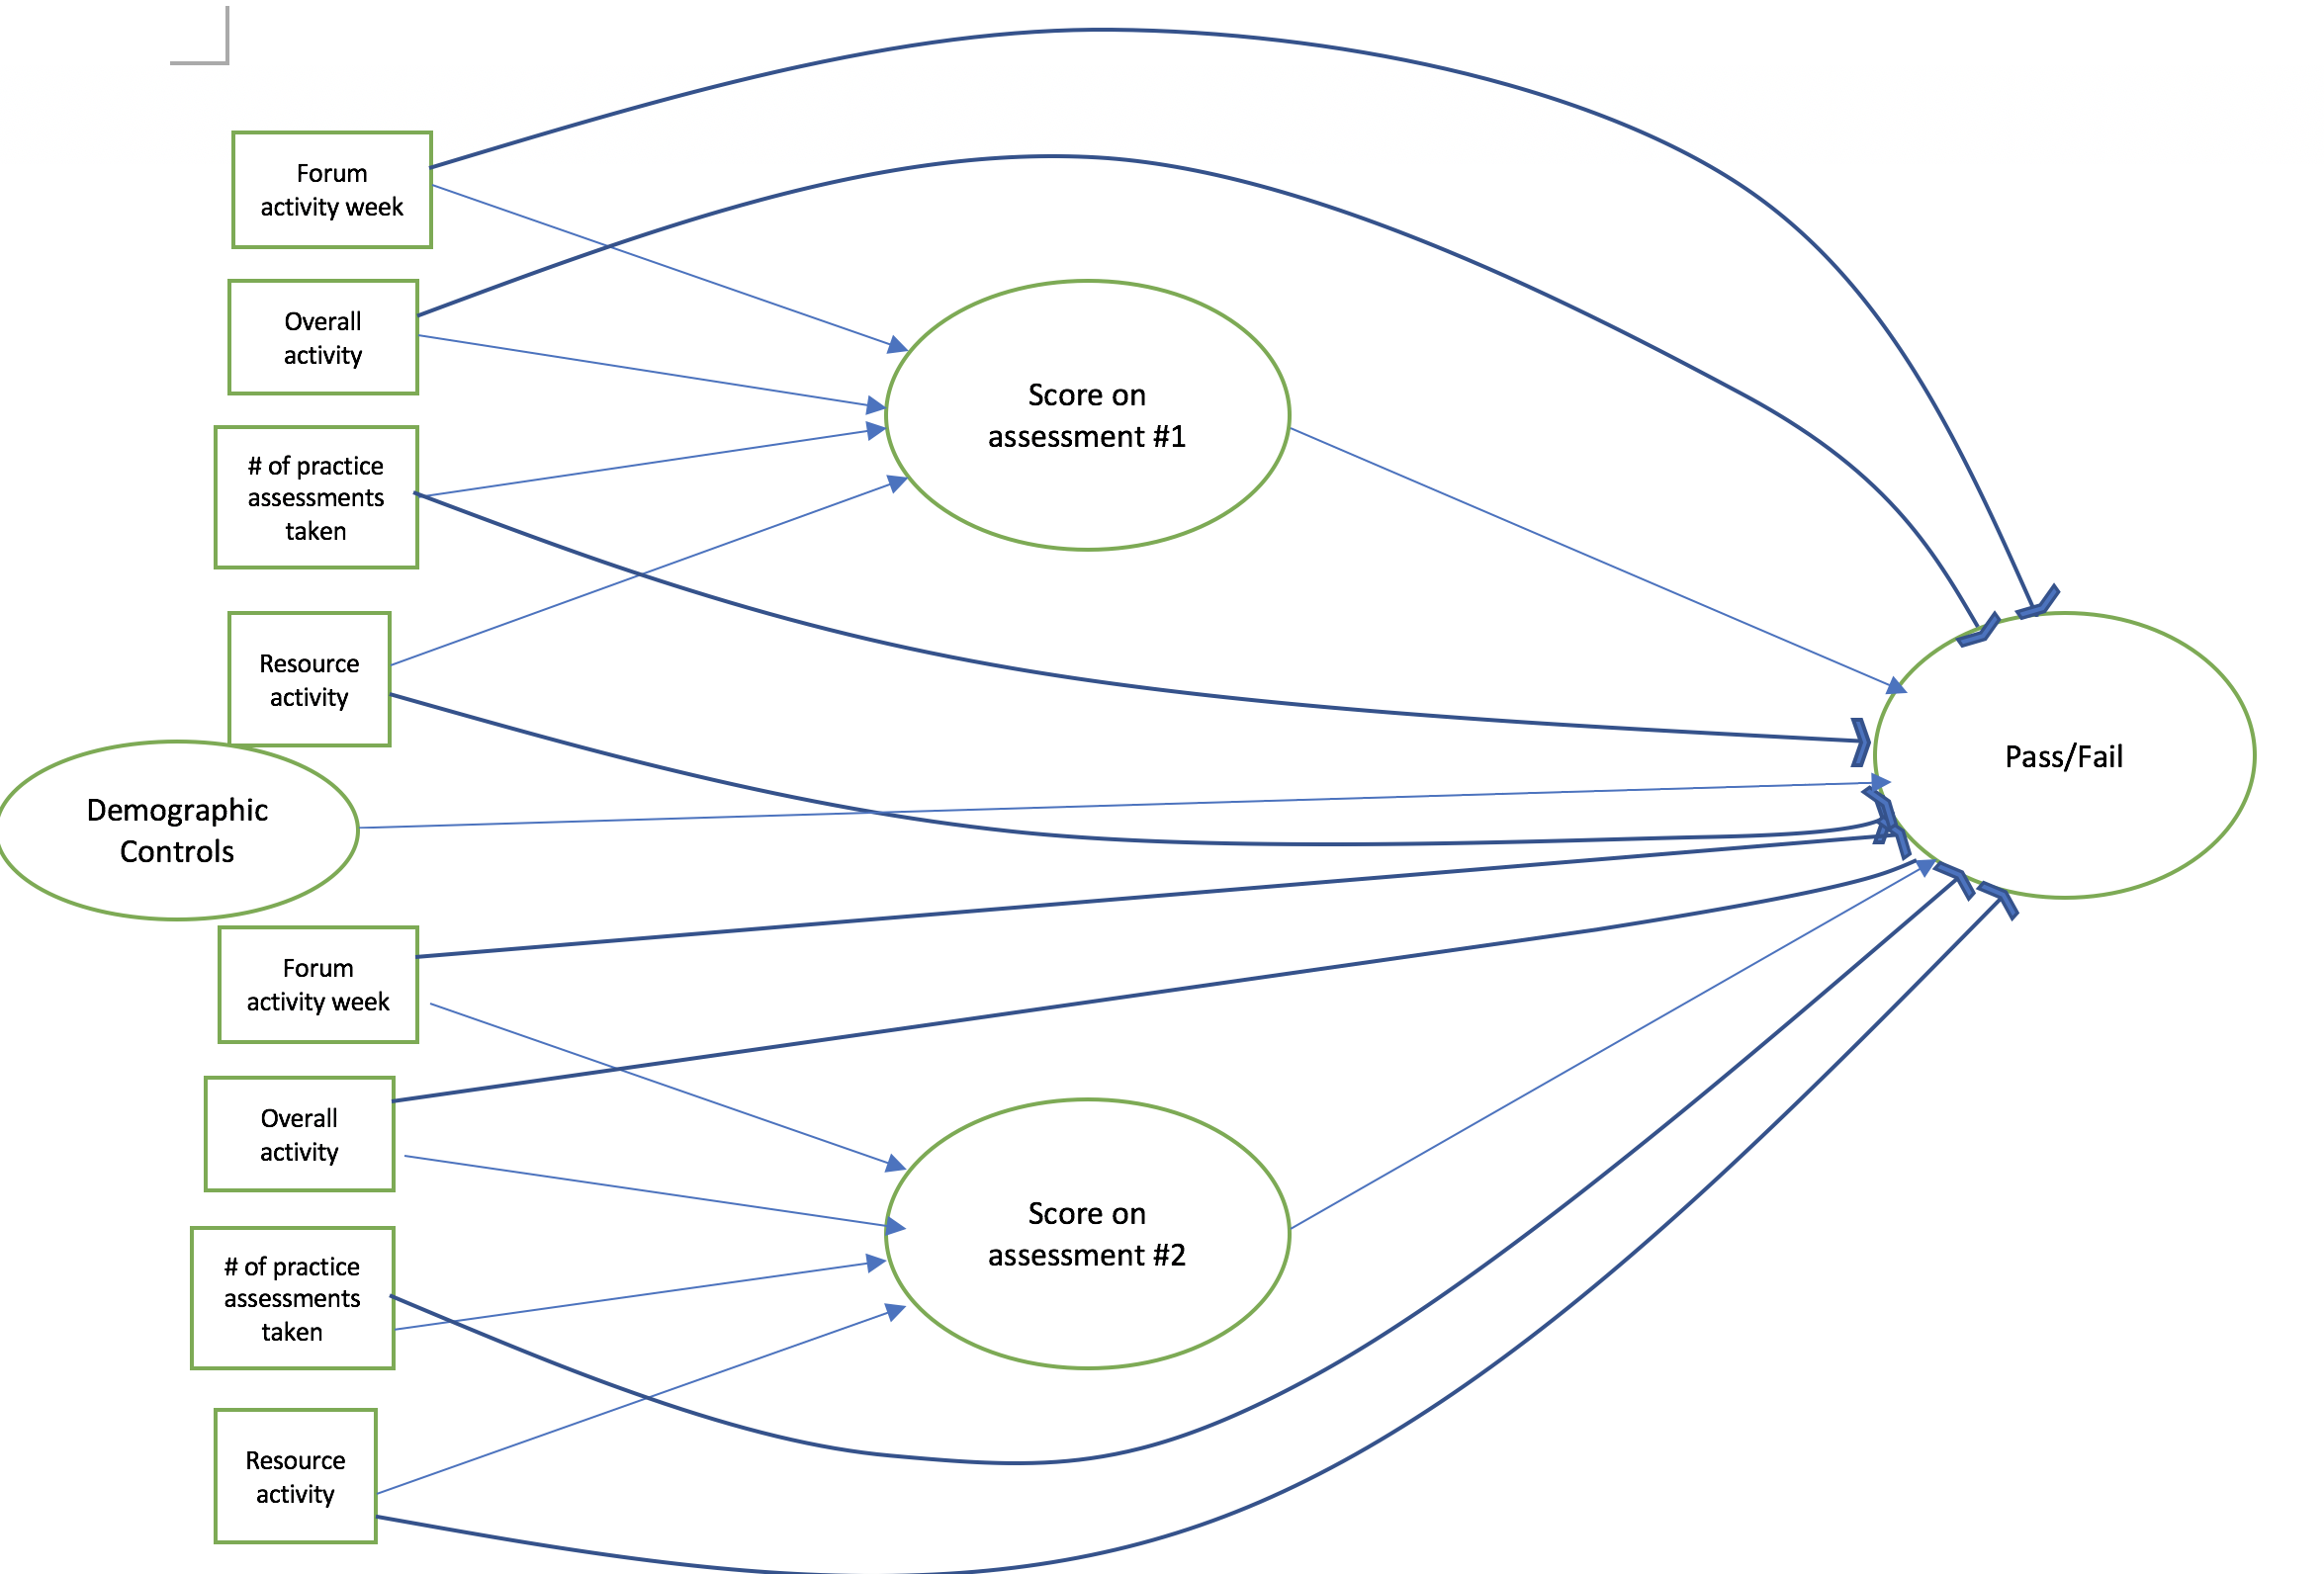
\includegraphics{sem_model_graph.png}
\caption{}
\end{figure}

\begin{Shaded}
\begin{Highlighting}[]
\NormalTok{mediation<-}\StringTok{ '}

\StringTok{score_TMA_group_3 ~ a0*activity_2 + a1*content_2 + a2*forum_2+ a3*resource_2 }
\StringTok{score_TMA_group_8 ~ b0*activity_7 + b1*content_7 + b2*forum_7+ b3*resource_7}
\StringTok{score_TMA_group_13 ~ c0*activity_12 + c1*content_12 + c2*forum_12+ c3*resource_12}
\StringTok{score_TMA_group_19 ~ d0*activity_18 + d1*content_18 + d2*forum_18+ d3*resource_18}
\StringTok{score_TMA_group_24 ~ e0*activity_23 + e1*content_23 + e2*forum_23+ e3*resource_23}

\StringTok{final_result~ f*score_TMA_group_3 +g*score_TMA_group_8+ h*score_TMA_group_13 +i*score_TMA_group_19 +j*score_TMA_group_24 + k*gender + l*imd_band + m*num_of_prev_attempts+n*studied_credits + o*disability}

\StringTok{indirect_activity2 := a0*f}
\StringTok{indirect_content2 := a1*f}
\StringTok{indirect_forum2 := a2*f}
\StringTok{indirect_resource2 := a3*f}

\StringTok{indirect_activity7 := b0*g}
\StringTok{indirect_content7 := b1*g}
\StringTok{indirect_forum7 := b2*g}
\StringTok{indirect_resource7 := b3*g}

\StringTok{indirect_activity12 := c0*h}
\StringTok{indirect_content12 := c1*h}
\StringTok{indirect_forum12 := c2*h}
\StringTok{indirect_resource12 := c3*h}

\StringTok{indirect_activity18 := d0*i}
\StringTok{indirect_content18 := d1*i}
\StringTok{indirect_forum18 := d2*i}
\StringTok{indirect_resource18 := d3*i}

\StringTok{indirect_activity23 := e0*j}
\StringTok{indirect_content23 := e1*j}
\StringTok{indirect_forum23 := e2*j}
\StringTok{indirect_resource23 := e3*j}
\StringTok{'}

\NormalTok{res<-}\KeywordTok{sem}\NormalTok{(mediation, }\DataTypeTok{data=}\NormalTok{sem, }\DataTypeTok{ordered=} \KeywordTok{c}\NormalTok{(}\StringTok{'final_result'}\NormalTok{, }\StringTok{'gender'}\NormalTok{, }\StringTok{'disability'}\NormalTok{))}
\CommentTok{#str(sem$gender)}
\CommentTok{#table(sem$content_group_3)}
\KeywordTok{summary}\NormalTok{(res)}
\end{Highlighting}
\end{Shaded}

Below are the truncated results of my mediation model where I only
include significant effects

\begin{Shaded}
\begin{Highlighting}[]
\CommentTok{# Defined Parameters:}
\CommentTok{#                        Estimate  Std.Err  z-value  P(>|z|)}
\CommentTok{#     content week 7       0.000    0.000    2.151    0.031}
\CommentTok{#     forum week 7         0.001    0.000    7.486    0.000}
\CommentTok{#     resources week 7     0.000    0.000    4.228    0.000}
\CommentTok{#     activity week 12     0.001    0.000    4.611    0.000}
\CommentTok{#     activity week 18     0.002    0.000    8.415    0.000}
\CommentTok{#     content week 18      0.001    0.000   10.004    0.000}
\CommentTok{#     resources week 18    0.000    0.000    4.764    0.000}
\CommentTok{#     activity week 23     0.002    0.000   15.191    0.000}
\CommentTok{#     content week 23      0.001    0.000   38.287    0.000}
\end{Highlighting}
\end{Shaded}

The indirect effects demonstrate significant pathways for mediation. For
instance, the positive and significant effect for content week 7
indicates that a students total activity on content modules from week
1-7 significantly effected their scores for their assessment on week 8,
which then also significantly effected their liklihood of passing or
failing.

From the above mediation results, we can infer several patterns:

\begin{enumerate}
\def\labelenumi{\arabic{enumi}.}
\tightlist
\item
  Significant mediation paths from online interactivity -\textgreater{}
  assessments -\textgreater{} pass/failing tend to exist more during the
  middle of the course than the begining or the end. This suggests that
  intervention, particularly through increased activity on online
  modules is only effective during the middle of courses. At the
  begining and end of courses, intervention through increased online
  activity may be to early or to late to significanlty affect student
  success outcomes.
\item
  Intervention for students should center around increasing online
  activity on content modules and overall activity (content modules
  includes activity like quizes, audio recording of lectures, etc. while
  overall activity is the amount of times students visit homepages,
  subpages, and other pages that may link to resources). The mediation
  models show that these effects significatly improve assessment
  outcomes, which in turn, increases a student's liklihood of passing.
  Conversly, activity like forums, and resources(e.g.~wikipedia,
  glossary, etc.) are not important intervention techniques.
\end{enumerate}

\subsection{Conclusion}\label{conclusion}

As personal/online learning continues to grow in popularity, it is
important to understand the factors that shape student success. In
particular, as data associated with online learning becomes more and
more available and robust, there is now an important opportunity to
identify intervention techniques to prevent student failure. In this
project, I used structural equation modeling to test how student
assessments scores mediated the relationship between different online
interactivity modules and the liklihood of students passing the course.
\textbf{I find that the best course of intervention for students as risk
for failure is to utilize encourage increased activity on content
modules and overall activity. In particular, this most effective during
the middle of the courses, rather than the begining or the end of
courses}


\end{document}
